\section{Manual analysis}
\label{sec:manual_analysis}

Our systematicity and substitutivity results demonstrate that models are not behaving compositional according to a strict definition of compositionality.
However, we ourselves have argued that strict compositionality is not always appropriate to handle natural language.
A reasonable question to ask is thus: are the inconsistencies we marked as non-compositional actually incorrect?

\paragraph{Annotation setup} 
To address this question, we perform a manual analysis.
We annotate 900 inconsistent translation pairs of the systematicity and substitutivity tests to establish whether the inconsistencies are benign or concerning.
We consider four different types of changes:
\begin{enumerate}[noitemsep,topsep=0pt]
\item cases of \textit{rephrasing}, where both translations are equally (in)correct;
\item changes reflecting different interpretations of \textit{source ambiguities};
\item cases in which one of the two translations contains an \textit{error};
\item \textit{formatting} (mostly punctuation) changes.
\end{enumerate}
For substitutivity samples, we also annotate whether the changes are related to the translation of the synonym, where we distinguish cases where
\begin{enumerate}[noitemsep,topsep=0pt]
\item[i.] one of the synonym translations is incorrect;
\item[ii.] both are incorrect but in a different manner;
\item[iii.] both are correct but translated differently;
\item[iv.] one synonym remains untranslated.
\end{enumerate}
We annotate all changes observed per pair and report the relative frequency per class. 
We summarise the results, aggregated over different training set sizes and the three data types, in Figure~\ref{fig:manual_analysis_summary}.
For a more elaborate analysis and a breakdown per model and data type, we refer to Appendix~\ref{app:man_analysis}.

\begin{figure}
	\begin{subfigure}[b]{\columnwidth}
		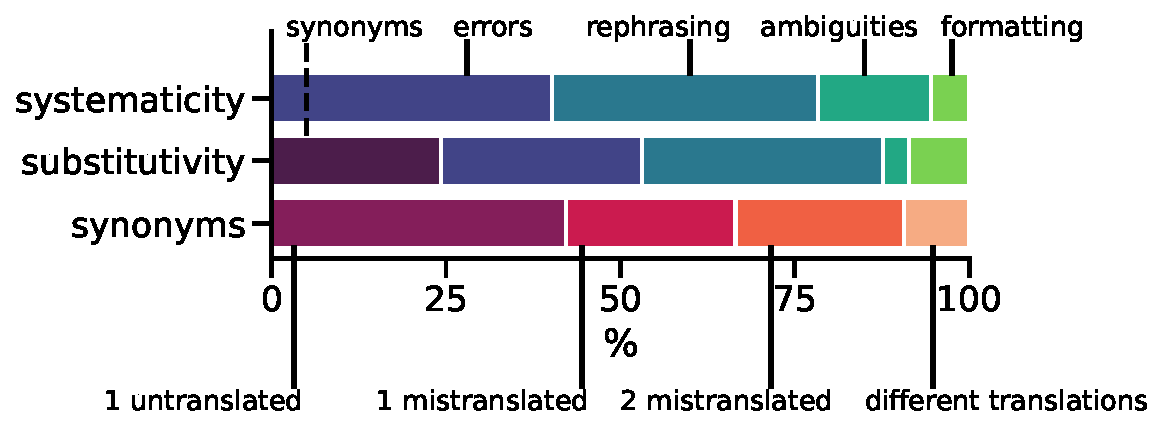
\includegraphics[width=\textwidth]{figures/analysis_appendix/summary_analysis.pdf}
	\end{subfigure}
	\caption{Relative frequencies of manually labelled inconsistencies in translations, averaged over data types and training set sizes.
	         The `synonyms' distribution further details the category `synonyms' from row two.}
	\label{fig:manual_analysis_summary}
	\vspace{-.3cm}
\end{figure}


\paragraph{Results}
In the systematicity test, 40\% of the marked inconsistencies reflects wrongfully translated parts in one of the two sentences, whereas 38\% contains examples of rephrasing, 16\% reflects ambiguities in the source sentences and 6\% is caused by formatting differences. 
For substitutivity, most inconsistencies are similar to the ones observed in systematicity: only 24\% involves the synonyms' translations, where one of them being untranslated was the most frequent category.
 
The distribution of these types of inconsistencies differ strongly per training data type.
For models trained on less data, inconsistencies are more likely to represent errors, whereas models trained on more data rephrase more often. 
This result emphasises that for lower-resource settings, being compositional is particularly relevant.

Another demonstration of this relevance comes from the observation that although models \textit{can} emit correct translations for nearly all synonyms,\footnote{Apart from the model with the small training dataset that cannot translate \exa{flautist} and \exa{ladybug}.}
they do not always do so, depending on the context.
To give a peculiar example: in ``The child admires the king that eats the \{doughnut, donut\}'', the snack was occasionally translated as ``ezel'' (\exa{donkey}).

\paragraph{Robustness and predictability}
Finally, we would like to stress that while rephrasing often might seem benign rather than concerning from the perspective of emitting adequate translations, its harmlessness still deserves some thought.
There is a fine line between rephrasing and mistranslating: whether ``the \textit{single largest} business establishment'' is referred to as ``de grootste'' (\exa{the largest}) or ``de enige grootste'' (\exa{the only largest}) may make or break a translation. 
Furthermore, if changes are unrelated to the contextual change (e.g. replacing ``soccer'' with ``football''), this can be undesirable from a robustness and reliability perspective.
This point becomes even more pronounced in cases where both translations are correct but have a different meaning.
To analyse the extent to which inconsistencies are actually unmotivated, we investigated if we could trace them back to the contextual change, in particular focusing on whether changing synonyms from British to American spelling or vice versa might trigger a change in style or tone.
We could not find evidence of such motivations, indicating that even correct cases of rephrasing were not caused by contextual changes that were \emph{necessary} to take into account.
